\chapter{Capa de datos}
\label{ch:datos}

El presente capítulo se ocupa de la capa de datos de la arquitectura del Perfil del estudiante. En particular, describe en detalle el proceso de extracción, transformación y carga al que los datos son sometidos. Se especifican las fuentes de datos utilizadas, el proceso de extracción de los datos del Ecosistema de analítica institucional, la transformación de los datos y la carga de los mismos en un sistema de almacenamiento que permita su consulta y análisis.

\section{Fuentes de datos}

En aras de que el Perfil del estudiante satisfaga su expectativa como núcleo de información académica y socioeconómica de los estudiantes de la Universidad de los Andes, es necesario que unifique la información que se encuentra dispersa en múltiples sistemas y formatos. En particular, se espera que el Perfil del estudiante sea capaz de reproducir, como mínimo, la información disponible en los sistemas de información académica de la Universidad, como Banner y Advise, así como información en el sistema de gestión financiera y en el portal de oferta de cursos. La tabla \ref{tab:fuentes_datos} detalla las fuentes de datos que deben ser integradas por el Perfil del estudiante, incluyendo el nombre formal de la fuente y una breve descripción de la información que contienen.

\begin{longtblr}[
		caption = {Fuentes de datos utilizadas por el Perfil del estudiante},
		label = {tab:fuentes_datos},
	]{
		colspec = {X[1,l] X[1,l] X[3,l]},
	}
	\hline
	\textbf{Nombre}               & \textbf{Nombre Formal}     & \textbf{Descripción}                                                                                                                                                                                                                                                                                                                                                                                                                                       \\
	\hline
	Banner                        & Ellucian Banner            & Sistema de planificación de recursos empresariales (ERP) diseñado para instituciones de educación superior. Gestiona procesos académicos y administrativos, incluyendo matrículas, registros académicos, finanzas y recursos humanos. \cite{banner} Almacena el registro académico completo de cada uno de los estudiantes de la Universidad en todos los niveles académicos, así como algunos de los antecedentes académicos del estudiante. \\
	Advise                        & Ellucian CRM Advise        & Sistema de gestión de relaciones con los estudiantes (CRM) que permite a las instituciones identificar y apoyar proactivamente a estudiantes en riesgo, facilitando intervenciones personalizadas para mejorar su éxito académico. \cite{advise}                                                                                                                                                                                                           \\
	Oferta de Cursos              & Portal de Oferta de Cursos & Plataforma web que permite a los estudiantes consultar los cursos disponibles en cada periodo académico, incluyendo información detallada sobre horarios y profesores. \cite{oferta_cursos}                                                                                                                                                                                                                                                                \\
	Sistema de Gestión Financiera &                            & Representación genérica de los sistemas contables y financieros de la universidad, en los que se maneja la información relacionada con becas, créditos educativos y pagos realizados por los estudiantes, así como datos socioeconómicos relevantes para la asignación de auxilios financieros.                                                                                                                                     \\
	\hline
\end{longtblr}

Para el acceso a la información contenida en estas fuentes de datos, la Universidad dispone de un Ecosistema de analítica institucional, cuyo propósito es precisamente facilitar el acceso a la información y la generación de conocimiento a partir de los datos. El Ecosistema tiene entre sus objetivos específicos \say{Entregar los datos con estándares de calidad y seguridad para suplir las necesidades de la Universidad}, \say{Hacer el uso de datos para garantizar una toma de decisiones informada} e \say{Impulsar una cultura de uso de datos en la Universidad} \cite{ecosistema}. El uso del Ecosistema evita tener que acceder directamente a las fuentes de datos, lo cual simplifica el proceso de extracción de datos y terceriza la responsabilidad de la consistencia de los mismos, al menos en su origen, a la Universidad. En la subsección \ref{subsec:extraccion} se detalla cómo se realiza la extracción de los datos del Ecosistema.

Como complemento a lo anterior, teniendo en mente la enorme responsabilidad que recae sobre el Ecosistema respecto a la calidad de los datos, lo cual es un aspecto crítico para que el Ecosistema pueda cumplir con sus objetivos y en efecto ser útil y confiable para las diversas dependencias de la Universidad, se realizó el esfuerzo de registrar en el apéndice \ref{ap:ecosistema} todos los problemas de calidad de los datos que se han encontrado en el Ecosistema y cómo se han abordado.
% TODO: Sí queda este apéndice?

\section{Proceso de extracción, transformación y carga}

La recuperación y el procesamiento de los datos se llevaron a cabo mediante un \textit{\gls{pipeline}} de analítica, implementado en cuadernos de \gls{Jupyter} con \gls{Python}, en colaboración con los estudiantes Santiago Martínez Novoa y Manuel Felipe Porras Tascón.
\footnote{Mi más sincero agradecimiento a ambos: a Manuel, en aquel momento estudiante de la Maestría en Ingeniería de la Información, por su valiosa labor al crear y trabajar inicialmente en el cuaderno; y a Santiago, entonces estudiante de Ingeniería de Sistemas y Computación, por tomar la posta, mejorar y mantener este trabajo. Su contribución fue fundamental para el desarrollo de este proyecto.}.
El pipeline de analítica realiza las tres etapas clásicas de un proceso de \gls{ETL}: extracción, transformación y carga de los datos. A cada una de estas etapas se le dedica una subsección en las siguientes líneas.


\subsection{Extracción de los datos}
\label{subsec:extraccion}

El proceso de extracción, a alto nivel, consiste en tomar la información relevante del Ecosistema de analítica institucional.

La información del Ecosistema se encuentra almacenada en \gls{Azure Blob Storage}, que es un servicio de almacenamiento de objetos en la nube de Microsoft Azure. Está distribuida en diversas cuentas de almacenamiento, cada una de las cuales contiene archivos en formato PARQUET y XLSX. Para el Perfil del estudiante, se hizo uso de diez de esos archivos, distribuidos en dos cuentas de almacenamiento. La figura \ref{fig:blob_storage} muestra la estructura de directorios y archivos en el Blob Storage que contienen la información relevante para el Perfil del estudiante.

\begin{figure}[h]
	\centering
	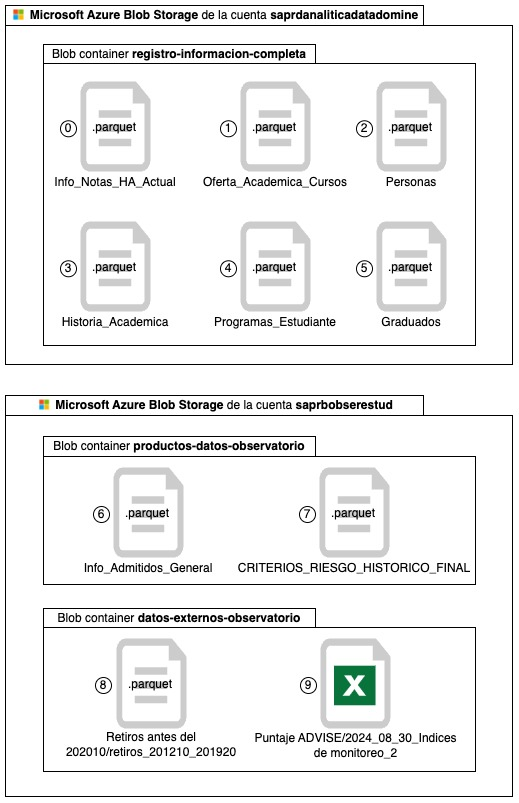
\includegraphics[width=0.7\textwidth]{img/blob_storage.jpg}
	\caption{Archivos fuente y estructura de directorios en \gls{Azure Blob Storage}}
	\label{fig:blob_storage}
\end{figure}

Cada uno de los archivos presentados en la figura \ref{fig:blob_storage} se carga en el cuaderno de \gls{Jupyter} y se extrae la información relevante para el Perfil del estudiante. La tabla \ref{tab:extraccion} detalla el orden en el que se realiza cada extracción, describe la información que se extrae y especifica el archivo fuente del cual se obtiene, empleando la numeración de los archivos definida en la figura \ref{fig:blob_storage}.

\begin{longtblr}[
		caption = {Extracción de datos},
		label = {tab:extraccion_datos},
	]{
		colspec = {X[1,l] X[2,l] X[4,l] X[2,l]},
	}
	\hline
	\textbf{Orden} & \textbf{Información}                               & \textbf{Descripción}                                                                                                                 & \textbf{Archivos fuente} \\
	\hline
	1              & Histórico académico                                & Información de las notas obtenidas por los estudiantes en cada una de las asignaturas que han cursado.                               & 0                        \\
	2              & Oferta \newline académica                          & Información de las asignaturas que se ofertan en cada uno de los semestres académicos.                                               & 1                        \\
	3              & Estudiantes                                        & Información básica de los estudiantes.                                                                                               & 2, 3, 6                  \\
	4              & Programas académicos                               & Información de los programas académicos en los que se encuentran inscritos los estudiantes.                                          & 4                        \\
	5              & Información \newline adicional \newline de retiros & Información sobre los retiros de los estudiantes para periodos anteriores al 2019-20, que no se encuentra en el Histórico académico. & 8                        \\
	6              & Graduados                                          & Información de los estudiantes que se han graduado.                                                                                  & 5                        \\
	7              & Criterios \newline de riesgo                       & Información de los criterios de riesgo que se utilizan para identificar a los estudiantes en riesgo académico.                       & 7                        \\
	8              & Advise                                             & Información de los estudiantes tomada de la plataforma Advise.                                                                       & 9                        \\
	\hline
\end{longtblr}

\subsection{Transformación de los datos}

El proceso de transformación asegura que los datos extraídos sean consistentes, completos y relevantes para los análisis requeridos en el proyecto. Esto implica la aplicación de múltiples pasos destinados a mejorar la calidad de los datos y a garantizar su integridad, tanto desde una perspectiva técnica como desde el contexto académico de la Universidad.

A continuación, se mencionan solo algunos de los pasos más relevantes que se llevaron a cabo como parte del proceso de transformación. No se presenta el detalle de la implementación, que es extenso y no aporta valor al proyecto, pero se puede encontrar en el cuaderno de \gls{Jupyter} que implementa el \gls{pipeline} de analítica. Es importante señalar que la implementación del cuaderno debe cambiar conforme los datos en el Ecosistema evolucionen, su estructura cambie o su calidad mejore (o empeore).

\begin{itemize}
	\item \textbf{Variables a utilizar} Tras cargar los datos, existen una serie de variables que no son relevantes para el análisis y que se eliminan. Notablemente, se eliminan las cédulas de ciudadanía de los estudiantes, pues a partir de este punto se identifican mediante el código estudiantil. Otros ejemplos de variables descartadas son aquellas con información detallada de los acudientes del estudiante y con las especifidades de nacionalidades y direcciones de residencia.
	\item \textbf{Consistencia} Se evalúa la consistencia de los datos en pos de unificar tipos y formatos, eliminando inconsistencias y redundancias. Esto es particularmente importante, ya que, al provenir de archivos en formato PARQUET y XLSX, las columnas no poseen un tipo de dato intrínseco, lo que impide garantizar que los datos presuntamente numéricos en efecto lo sean. Ejemplos simples de esto son la transformación del código estudiantil y del periodo a tipos numéricos. Recuérdese que el periodo académico se representa con un número entero que concatena al año y el periodo académico, verbigracia, 201910 representa el primer semestre del año 2019, que convencionalmente se escribe como 2019-10.
	\item \textbf{Validez} Se verifica la validez de los datos. Por ejemplo, se descartan registros con valores nulos en campos críticos como el código estudiantil o el periodo académico, pues resulta inviable realizar un análisis académico sin información de estos campos.
	\item \textbf{Unicidad} Se garantiza la unicidad de los datos, mediante la eliminación de registros duplicados.
	\item \textbf{Completitud y relevancia} Se completan los datos faltantes, asignando valores predeterminados a campos críticos como la calificación final de materias. Se separan los datos que son irrelevantes para los cálculos académicos, como las materias relacionadas con deportes; no se eliminan, pues luego se reincorporan para ser mostrados como materias en el Perfil del estudiante.
	\item \textbf{Indicadores académicos} Se crean columnas adicionales y se calculan indicadores académicos relevantes que no existen en las fuentes originales de los datos. Algunos indicadores notables son:
	      \begin{itemize}
		      \item Se asignan clasificaciones a los estudiantes en estados como \textit{ACTIVO}, \textit{INACTIVO} o \textit{DESERTOR}, considerando el tiempo transcurrido desde su última matrícula.
		      \item Se realiza el cálculo de los créditos aprobados, reprobados, retirados, pendientes e incompletos, tanto de forma global como segmentada por áreas específicas como matemáticas, física y materias de la carrera.
		      \item Se calcula el número de matrículas del estudiante. Este indicador representa el número de semestres completos que han sido pagados y matriculados. Se calcula con dos decimales, donde un semestre completo equivale a una matrícula; media matrícula equivale a 0.5 matrículas; y un cuarto de matrícula, un periodo intersemestral, una práctica académica u otros casos similares equivalen a 0.25 matrículas. Esto provee una medida de la inversión realizada en la educación del estudiante mucho más precisa que simplemente el semestre en el que se encuentra matriculado.
	      \end{itemize}
\end{itemize}

Naturalmente, el proceso de transformación es mucho más extenso y detallado que lo presentado aquí. Estos ejemplos solo ilustran lo que ocurre en el proceso.

\subsection{Carga de los datos}

Tras el proceso de transformación, es necesario cargar los datos transformados en un sistema de almacenamiento que permita su consulta y análisis, no solo por parte del Perfil del estudiante, sino para otros análisis por parte de la Vicedecanatura de Asuntos Estudiantiles de la Facultad de Ingeniería o de cualquier otra dependencia de la Universidad.

A causa de eso, el notebook genera varios archivos PARQUET que almacenan la información transformada, organizándola semánticamente en archivos distintos para facilitar su consulta y análisis. Estos archivos se almacenan en el contenedor de Azure Blob Storage que se muestra en la figura \ref{fig:blobs_generados}.

\begin{figure}
	\centering
	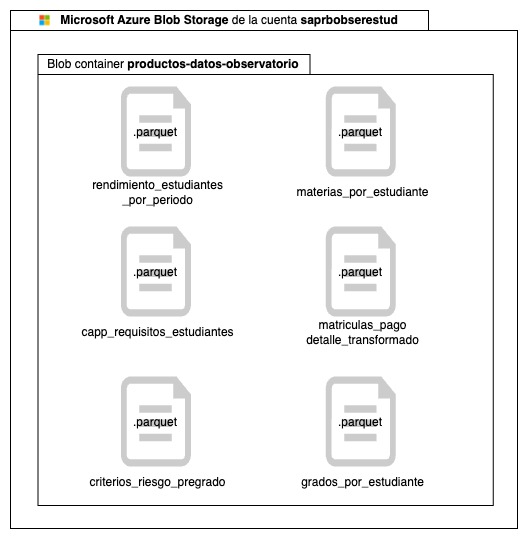
\includegraphics[width=0.7\textwidth]{img/blobs_generados.jpg}
	\caption{Archivos generados por el proceso de transformación}
	\label{fig:blobs_generados}
\end{figure}

La tabla \ref{tab:blobs_generados} detalla los archivos generados y la información que contienen, a pesar de que los nombres de los archivos son autoexplicativos. En favor de la claridad, para cada archivo se describe de qué manera se debe interpretar cada registro. 

\begin{longtblr}[
		caption = {Archivos generados por el proceso de transformación y su contenido},
		label = {tab:blobs_generados},
	]{
		colspec = {X[1,l] X[3,l]},
	}
	\hline
	\textbf{Archivo}                        & \textbf{Contenido}                                                                                                  \\
	\hline
	rendimiento\_estudiantes\_por\_periodo  & Contiene el rendimiento académico de los estudiantes. Cada registro consta de indicadores académicos calculados para un estudiante en un periodo académico específico. \\
	criterios\_riesgo\_pregrado             & Almacena información relacionada con los criterios de riesgo académico en programas de pregrado. Cada registro corresponde a un estudiante e indica qué criterios de riesgo cumple, en caso de cumplir alguno. \\
	capp\_requisitos\_estudiantes           & Registra los requisitos cumplidos y pendientes de los estudiantes para la formalización de su grado. Cada registro representa un estudiante y especifica los requisitos cumplidos y los que aún están pendientes. \\
	materias\_por\_estudiante               & Incluye el detalle de las materias inscritas y su información correspondiente por estudiante y periodo académico. Cada registro representa un curso inscrito por un estudiante en un periodo académico. \\
	matriculas\_pago\_detalle\_transformado & Presenta las especificidades de las matrículas y los pagos realizados por los estudiantes tras la transformación de datos. Cada registro corresponde a un pago realizado por una fuente de financiación que cubre total o parcialmente la matrícula de un estudiante en un periodo académico. \\
	grados\_por\_estudiante                 & Contiene información sobre los grados obtenidos por los estudiantes, incluyendo fechas y programas. Cada registro corresponde a un grado obtenido por un estudiante. \\
	\hline
\end{longtblr}

Estos archivos se crean con el propósito de proporcionar la información que se almacena en la base de datos de \gls{PostgreSQL} del \gls{API REST}, que se describe en el capítulo \ref{ch:logica}. No obstante, su potencial de aplicación es considerablemente más amplio. Lamentablemente, los detalles del valioso uso que se les ha dado no pueden ser revelados en este documento.
